% Тут используется класс, установленный на сервере Papeeria. На случай, если
% текст понадобится редактировать где-то в другом месте, рядом лежит файл matmex-diploma-custom.cls
% который в момент своего создания был идентичен классу, установленному на сервере.
% Для того, чтобы им воспользоваться, замените matmex-diploma на matmex-diploma-custom
% Если вы работаете исключительно в Papeeria то мы настоятельно рекомендуем пользоваться
% классом matmex-diploma, поскольку он будет автоматически обновляться по мере внесения корректив
%
\documentclass{matmex-diploma-custom}
\begin{document}
% Год, город, название университета и факультета предопределены,
% но можно и поменять.
% Если англоязычная титульная страница не нужна, то ее можно просто удалить.
\filltitle{ru}{
    chair              = {Кафедра Системного Программирования},
    title              = {Автоматизация сборки и публикации плагинов к ReSharper для анализа встроенных языков},
    % Здесь указывается тип работы. Возможные значения:
    %   coursework - Курсовая работа
    %   diploma - Диплом специалиста
    %   master - Диплом магистра
    %   bachelor - Диплом бакалавра
    type               = {coursework},
    position           = {студента},
    group              = 242,
    author             = {Григорьев Сергей Романович},
    supervisorPosition = {магистр информационных технологий, ст. преп.},
    supervisor         = {Григорьев С.\,В.},
%   university         = {Санкт-Петербургский Государственный Университет},
    faculty            = {Математико-механический факультет},
%   city               = {Санкт-Петербург},
%   year               = {2013}
}
\maketitle
\tableofcontents
% У введения нет номера главы
\section*{Введение}

Обычно при разработке сложных программ используется более одного языка программирования. В таких ситуациях говорят об основном и встроенных языках.

Встроенный язык - язык, команды которого выполняются из базового языка. Обычно это предметно-ориентированные языки (специализированные под конкретную область применения). Встроенный язык расширяет функциональные возможности языка общего назначения при его использовании в области, специфичной для встроенного языка.

Код встроенного в C\# языка представляется компилятору в виде строкового выражения и, как следствие, невозможно провести его анализ до момента исполнения. Данную проблему разрешает статический анализ встроенных языков.
Код на встроенном языке генерируется динамически (путем конкатенации строк, подстановки значений в шаблоны, в условных операторах, циклах и т.д.). В такой ситуации сопровождение кода и поиск ошибок в коде значительно усложняется, поскольку среды разработки ПО зачастую не предоставляют средств для подсветки синтаксиса, рефакторинга и т.п. в строковых выражениях.

В такой ситуации полезным оказываются программные продукты, которые позволяют провести лексический и синтаксический анализ встроенного языка и добавить в среду разработки функционал, упрощающий работу с ним (подсветка синтаксиса, обнаружение ошибок и опечаток до компиляции и т.д.).

Одним из таких продуктов является модульный инструмент YaccConstructor (далее по тексту - YC) \cite{yc}. Он позволяет создавать лексические и синтаксические анализаторы. На его базе разработаны плагины к ReSharper (далее по тексту - R\#) \cite{resharper} - плагину к среде разработки Microsoft Visual Studio (далее по тексту - MSVS). Данные модули позволяют анализировать код на языке Transact-SQL (далее по тексту - TSQL) и языке арифметических выражений Calc, встроенный в код на языке C\#.

Модульная структура имеет свои преимущества и недостатки. К преимуществам относятся:

\begin{itemize}
\item
упрощение командной разработки;
\item
упрощение тестирования и поиска ошибок;
\item
возможность разработки на нескольких основных языках программирования;
\item
возможность использования только тех модулей, функциональность которых требуется;
\item
переиспользование компонентов системы для решения других задач.
\end{itemize}

Одним из значительных недостатков модульной структуры программного продукта является усложнение процесса его сборки. Для решения данной задачи существует ряд программных продуктов, позволяющих автоматизировать весь процесс сборки, тестирования и публикации. В YC используется система для автоматизации сборки FAKE. Она позволяет полностью автоматизировать весь процесс сборки, тестирования, публикации, обновления версий.

Для распространения бинарных пакетов также существует ряд решений. Одним из них является NuGet \cite{nuget}. Он позволяет публиковать бинарные пакеты, разрешать зависимости между ними, контролировать версии, что значительно упрощает как работу разработчиков, так и использование продукта конечными пользователями. Именно он используется в качестве менеджера плагинов к R\#, и если разработчик плагина хочет опубликовать свой продукт, ему рекомендуется воспользоваться именно NuGet.

Таким образом, выделение модулей для анализа встроенных языков из YC, компоновка их по бинарным пакетам и размещение в репозитории плагинов R\# значительно упростит их дальнейшую разработку, а также использование конечными пользователями.

\section{Постановка задачи}

Целью данной работы является упрощение и систематизация процесса разработки плагинов к R\# для анализа встроенных языков в строковых выражениях в коде языка C\#.

Для достижения цели поставлены следующие задачи:

\begin{enumerate}
\item
проанализировать структуру YC;
\item
выделить в YC плагины для анализа встроенных языков (YC.SEL.Plugins.Core, содержащий общую логику работы, YC.SEL.Plugins.Calc и YC.SEL.Plugins.TSQL, содержащие логику анализа соответствующих языков);
\item
сформировать из плагинов бинарные пакеты;
\item
встроить процесс сборки и публикации данных пакетов в систему сборки FAKE \cite{fake}, используемую в проекте YC;
\item
реализовать возможность отображения установленных на данный момент плагинов в меню R\#.
\end{enumerate}

\section{Обзор существующих решений}

\subsection{Решения для распространения пакетов}

Пакет - это набор взаимосвязанных компонентов, предназначенных для решения конкретной задачи, а также служебных данных, необходимых для его использования.

Для распространения пакетов и слежения за зависимостями используются менеджеры пакетов - программы, позволяющие корректно установить необходимый пакет, а так же пакеты, которые ему требуются, удалить пакет вместе с зависящими от него пакетами, обновить установленные в системе пакеты при появлении новой версии и т.д. Такой подход широко распространен в UNIX-подобных операционных системах для управления установленными на компьютере программами. Для этих целей там используются такие системы управления пакетами, как:

\begin{enumerate}
\item
RPM (используется в Red Hat/Fedora и производных от них дистрибутивах);
\item
dpkg (используется в Debian и производных от него дистрибутивах);
\item
Portage (используется в Gentoo и производных от него дистрибутивах).
\end{enumerate}

В операционных системах семейства Windows нет предустановленной системы управления пакетами. Но существуют решения, добавляющие туда подобный функционал. Например, менеджер пакетов Chocolatey.

Все приведенные здесь менеджеры пакетов обладают схожим функционалом: возможность создания репозиториев, сборки и публикации пакетов, установки и разрешения зависимостей, контроль обновлений и т.д. Пакет в них представляет из себя архив какого-либо формата, содержащий в себе бинарные файлы и метаданные, описывающие пакет, его зависимости и т.п.

Однако у Portage есть существенные отличия. В Portage почти все устанавливаемые программы собираются на компьютере конечного пользователя из исходных кодов. В Portage нет пакетов, вместо них используются ebuild-файлы, которые описывают, где находятся файлы с исходными кодами, как их правильно собирать и куда устанавливать. Также Portage поддерживает весь основной функционал, который есть у трех других вышеописанных менеджеров пакетов. Преимуществом такого подхода является ускорение работы программ, т.к. они могут быть оптимизированы для работы на конкретном компьютере при компиляции. Несмотря на отсутствие пакетов, как в остальных приведенных здесь менеджерах (отсутствие архива с самой программой), Portage решает те же задачи, поэтому его упоминание уместно в рамках данной работы.

Менеджер пакетов NuGet, используемый в среде разработки MSVS и в плагине к ней - R\# - как средство для установки плагинов и библиотек, а также используемый в проекте YC для размещения пакетов, обладает схожим функционалом с RPM, dpkg и Chocolatey. В отличие от других описанных в этом разделе менеджеров пакетов, NuGet, в силу специфики его применения (как менеджера пакетов с библиотеками в среде разработки), позволяет устанавливать пакеты индивидуально для каждого проекта в среде MSVS. При использовании для установки пакетов R\# устанавливает расширения глобально (для всех проектов).

\subsection{Решения для автоматизации сборки}

Сборка больших программных продуктов является сложным процессом. Недостаточно просто воспользоваться компилятором. Требуется подготовить проект к сборке, настроить его, установить правильную версию, скомпилировать его компоненты в правильной последовательности, произвести тестирование, подготовить получившиеся бинарные файлы к публикации и т.п. Для этих целей можно использовать скрипты встроенной в операционную систему оболочки, например .bat скрипты в ОС семейства Windows или .sh скрипты в Unix-подобных ОС. Но гораздо удобнее воспользоваться системой автоматизированной сборки. Такие системы предоставляют готовый набор методов для простого и быстрого создания сборочных скриптов.

Примерами подобных систем являются:

\begin{enumerate}
\item
GNU make - система сборки, используемая большинством программ в ОС семейства Linux;
\item
Apache Ant - платформонезависимая версия make, в которой файлы конфигурации проекта используют формат XML;
\item
FAKE (F\# make) - система сборки, использующая скрипты на языке F\# с расширенным синтаксисом.
\end{enumerate}

Во всех приведенных выше системах сборки ключевым понятием является цель (target). Целью может быть какой-либо этап сборки (например, при установке программного обеспечения из исходных кодов в ОС семейства Linux используется команда “make install”, что означает “запустить цель install из файла конфигурации по умолчанию (Makefile)”). Итоговым результатом работы системы является последовательное или выборочное выполнение целей.

Проект YC использует именно FAKE для сборки. Данная система использует скрипты на языке F\#, а также позволяет подключать любые .NET-библиотеки и использовать их функционал. Это позволяет написать сборочные скрипты для проектов любой сложности.

\section{Реализация}

На момент начала работы проект YC уже содержал в себе плагины для анализа встроенных языков. Их исполняемые файлы находились в одной директории с остальными исполняемыми файлами.

Во время работы было проведено исследование проекта YC. Были выделены 3 логические компоненты, связанные с анализом встроенных языков:

\begin{enumerate}
\item
YC.SEL.Plugins.Core - главный плагин, содержащий общий функционал, требующийся двум другим плагинам;
\item
YC.SEL.Plugins.TSQL - плагин, отвечающий за анализ и подсветку синтаксиса в строках, содержащих запросы на языке TSQL;
\item
YC.SEL.Plugins.Calc - плагин, отвечающий за анализ и подсветку синтаксиса в строках, содержащих арифметические выражения.
\end{enumerate}

Были написаны конфигурационные файлы для формирования пакетов Nuget. В итоге получились следующие пакеты и их зависимости:

% IMAGE HERE ------------------------------------------------------------------

\begin{figure}[h!]
	\center{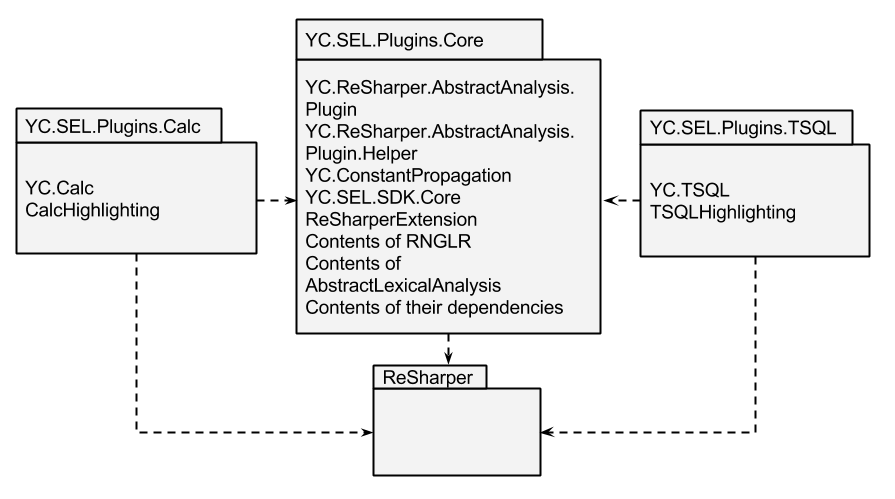
\includegraphics[width=1\linewidth]{dia.png}}
	\caption{Диаграмма пакетов}
\end{figure}

Во время интеграции данных пакетов в систему сборки YC столкнулись со следующими проблемами:

\begin{itemize}
\item
сборочные скрипты управляли сборкой только одного NuGet-пакета, все было настроено только на работу с ним и не сочеталось с необходимостью обрабатывать сразу несколько пакетов по одному алгоритму;
\item
обновление версий пакетов и исполняемых файлов было выборочным и нецентрализованным.
\end{itemize}

Для решения данных проблем были выполнены следующие изменения в проекте YC:

\begin{itemize}
\item
конфигурационные файлы NuGet-пакетов размещены в отдельной директории, реализована их однотипная обработка с помощью скриптов, включая редактирование конфигурационных файлов пакетов с целью обновить версию пакета, упаковку пакетов и размещение их в репозитории MyGet - одном из репозиториев NuGet;
\item
создан файл VERSION в корневой директории проекта, в нем хранится версия текущей работающей сборки, скрипты используют информацию из данного файла для обновления версии во всем проекте.
\end{itemize}

Для реализации отображения установленных на данный момент плагинов в меню R\# был модифицирован код плагина YC.SEL.Plugins.Core. В меню отображается, сколько и каких плагинов установлено, либо указывается, что не установлен ни один.


% У заключения нет номера главы
\section*{Заключение}

За время выполнения работы достигнуты следующие результаты:

\begin{enumerate}
\item
исследован проект YC, выделены компоненты для анализа встроенных языков;
\item
выделены 3 плагина для анализа встроенных языков;
\item
скомпанованы, собраны и опубликованы в репозитории MyGet 3 пакета для анализа встроенных языков:
\begin{enumerate}
\item
YC.SEL.Plugins.Core;
\item
YC.SEL.Plugins.TSQL;
\item
YC.SEL.Plugins.Calc;
\end{enumerate}
\item
сборка и публикация пакетов встроена в автоматизированную систему сборки прокета YC;
\item
реализовано отображение установленных на данный момент плагинов в меню R\#.
\end{enumerate}

Результаты работы размещены в репозиториях https://github.com/YaccConstructor/YaccConstructor и https://github.com/YaccConstructor/Build.Tools от имени пользователя unstope.

\bibliographystyle{ugost2008ls}
\bibliography{coursework.bib}

\end{document}
